\chapter{X-ray}
\label{ch:x_ray}

% Chapter-opening illustrated modality infographic.
\begin{center}
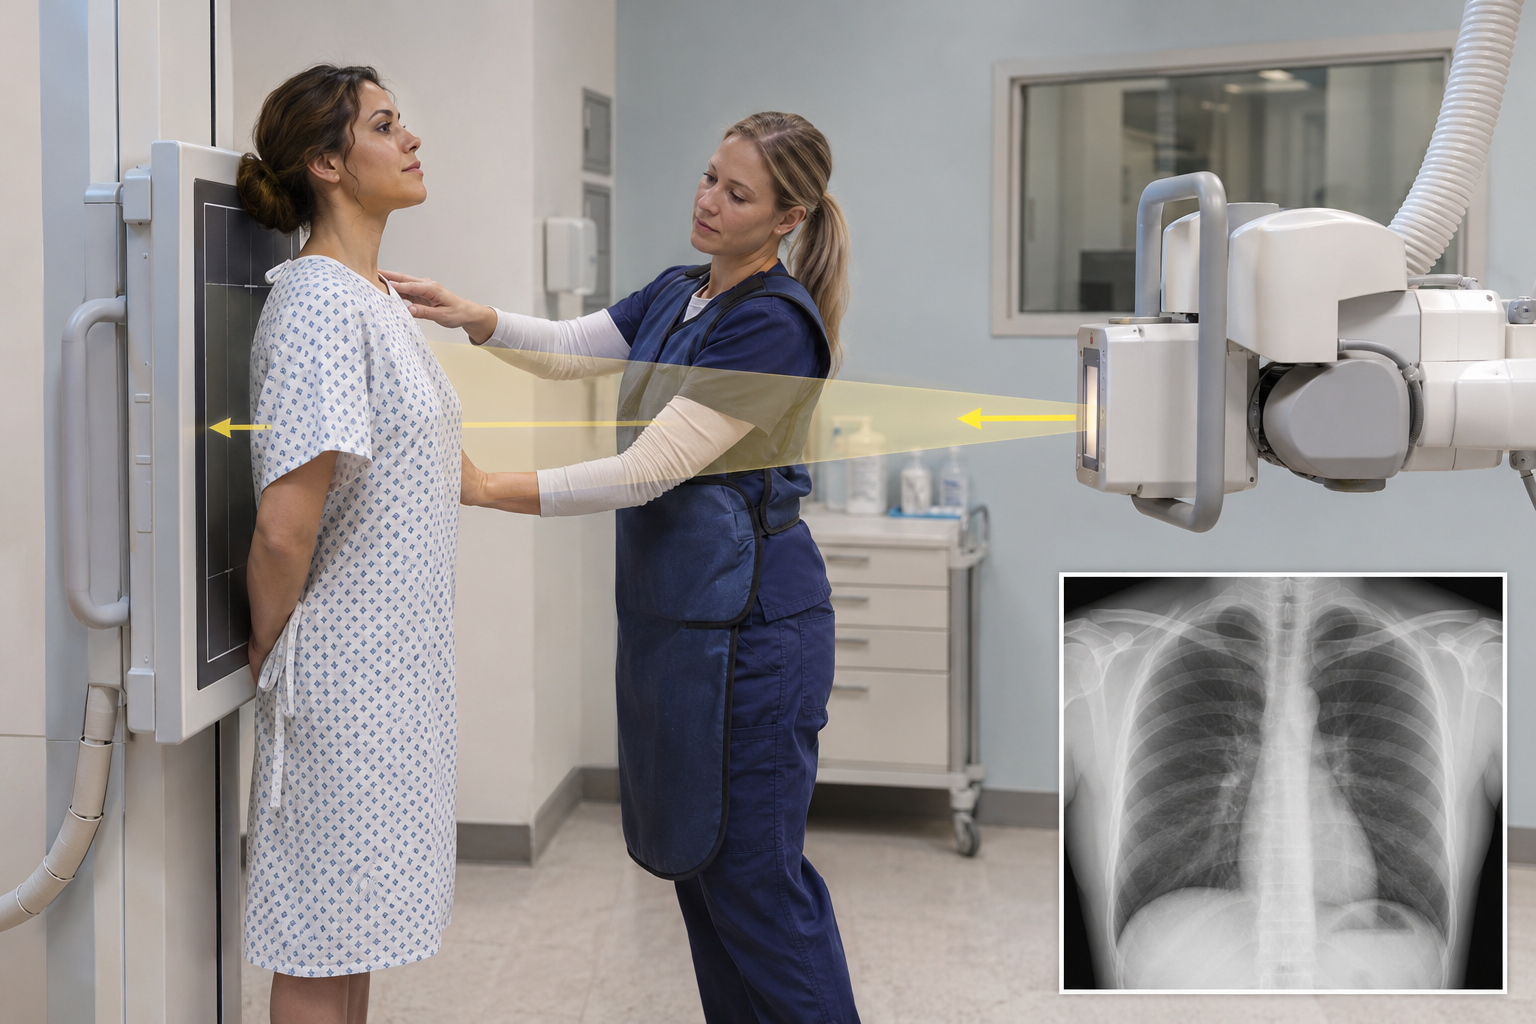
\includegraphics[width=\textwidth,keepaspectratio]{modalities/infographics/x_ray_realistic.png}
\end{center}
\begin{center}\footnotesize Projection radiography records the summed X-ray attenuation along each beam path, so anatomy overlaps and positioning affects visibility. AI-generated illustration; radiograph inset is not a patient study.\end{center}

\section{Overview}
Conventional plain X-ray imaging, also called radiography, produces two-dimensional projection images by passing X-rays through the body to a detector. Dense structures such as bone absorb more X-rays and appear relatively white; air appears dark, while soft tissues appear in shades of grey.

This chapter covers plain projection radiographs of the chest, skeleton, abdomen and urinary tract. A radiograph can reveal the shape of a fracture, show how far joint damage has progressed or suggest the cause of an obstruction. What it reveals depends on the projection, the tissue involved and the stage of disease.

\section{Selected applications of plain radiography}
The numbered entries pair each condition, injury or finding with an example of its appearance. Some appearances have several possible causes. For example, a chest film can show fluid in the pleural space, but identifying blood in that fluid requires additional evidence.

\subsection{Chest X-rays}
\begin{enumerate}[leftmargin=*,itemsep=0.45em,topsep=0.4em]
\item \textbf{Acute respiratory distress syndrome (ARDS).}\par\noindent\textbf{Symptoms:} Acute hypoxemia and respiratory distress prompt bedside chest imaging.\par\noindent\textbf{Clinical Features:} Bilateral opacities, distribution, interval change, and signs of pleural fluid or cardiac enlargement that may suggest another or additional cause.\par\noindent\textbf{Role and sufficiency:} The film supports assessment and monitoring but cannot diagnose ARDS by itself; clinicians combine timing, oxygenation, clinical cause, and exclusion of hydrostatic edema.
\item \textbf{Asbestosis.}\par\noindent\textbf{Symptoms:} Progressive exertional breathlessness or cough in someone with occupational asbestos exposure may prompt imaging.\par\noindent\textbf{Clinical Features:} Basal interstitial markings and pleural plaques; plaques show exposure but do not prove pulmonary fibrosis.\par\noindent\textbf{Role and sufficiency:} Radiography can reveal established disease, but a normal or equivocal film does not exclude early fibrosis. HRCT and exposure history are often needed for characterization.
\item \textbf{Atelectasis.}\par\noindent\textbf{Symptoms:} New breathlessness or low oxygen levels, reduced breath sounds, or postoperative respiratory changes may prompt a chest radiograph; small areas of collapse can also be incidental.\par\noindent\textbf{Clinical Features:} A denser region accompanied by volume loss. Fissure displacement and crowded bronchovascular markings are direct clues; hilar or mediastinal shift toward the affected side, an elevated hemidiaphragm, and compensatory expansion of nearby lung support the interpretation. Air bronchograms may remain visible when bronchi are open, so they do not by themselves exclude collapse.\par\noindent\textbf{Role and sufficiency:} Chest X-ray is usually the initial imaging test and often identifies substantial lobar collapse when these signs are visible. It does not reliably identify the cause; CT or bronchoscopy may be needed when collapse is unexplained, persistent, recurrent, or suspicious for an obstructing lesion. \textbf{Diagnostic performance:} There is no single success percentage for atelectasis across all presentations. Subsegmental or early collapse may be subtle or occult, particularly on a portable single-view study. See the \href{https://www.ncbi.nlm.nih.gov/books/NBK621651/}{NCBI chest radiograph review} and \href{https://pmc.ncbi.nlm.nih.gov/articles/PMC10902601/}{Fleischner Society thoracic imaging glossary}.
\item \textbf{Cardiomegaly.}\par\noindent\textbf{Symptoms:} Breathlessness, edema, or a suspected change in heart size may lead to a chest film.\par\noindent\textbf{Clinical Features:} An enlarged cardiac silhouette, while checking projection, rotation, and inspiration; AP portable views magnify the heart.\par\noindent\textbf{Role and sufficiency:} Radiography can suggest enlargement but cannot measure chamber size or establish its cause. Echocardiography is used when cardiac structure or function needs assessment.
\item \textbf{Congestive heart failure.}\par\noindent\textbf{Symptoms:} Acute breathlessness, shortness of breath when lying flat, or edema may prompt a chest radiograph for pulmonary congestion and alternative diagnoses.\par\noindent\textbf{Clinical Features:} Vascular redistribution, interstitial or alveolar edema, pleural effusions, and cardiac silhouette, interpreted together.\par\noindent\textbf{Role and sufficiency:} The film supports but neither confirms nor excludes heart failure; examination, biomarkers, and echocardiography may be needed.
\item \textbf{Diaphragmatic hernia.}\par\noindent\textbf{Symptoms:} Respiratory distress, chest symptoms, or an incidental thoracic opacity may raise suspicion.\par\noindent\textbf{Clinical Features:} Bowel gas, an air-fluid level, or abdominal viscera above the diaphragm.\par\noindent\textbf{Role and sufficiency:} A radiograph can reveal a conspicuous hernia, but CT or other targeted imaging may be needed to define the defect and contents, especially when the film is equivocal.
\item \textbf{Emphysema.}\par\noindent\textbf{Symptoms:} Chronic breathlessness, cough, or suspected COPD may lead to chest radiography.\par\noindent\textbf{Clinical Features:} Hyperinflation, flattened diaphragms, and increased retrosternal airspace.\par\noindent\textbf{Role and sufficiency:} These are supportive signs, not a measure of airflow obstruction; spirometry establishes COPD, while CT better characterizes emphysema.
\item \textbf{Foreign body aspiration.}\par\noindent\textbf{Symptoms:} Sudden choking or cough, unilateral wheeze, or persistent focal respiratory symptoms—particularly in a child—may prompt imaging.\par\noindent\textbf{Clinical Features:} A radiopaque object, unilateral air trapping, atelectasis, or recurrent focal infection.\par\noindent\textbf{Role and sufficiency:} Many aspirated objects are radiolucent, so a normal film cannot rule out aspiration. Bronchoscopy may be required when clinical suspicion remains high.
\item \textbf{Hemothorax.}\par\noindent\textbf{Symptoms:} Chest trauma with breathlessness, chest pain, or circulatory compromise prompts rapid assessment for pleural blood.\par\noindent\textbf{Clinical Features:} Pleural opacity or layering fluid; a supine film may show only diffuse haziness.\par\noindent\textbf{Role and sufficiency:} X-ray detects larger collections but cannot reliably distinguish blood from other pleural fluid. Ultrasound or CT clarifies uncertain cases and injury extent.
\item \textbf{Lung abscess.}\par\noindent\textbf{Symptoms:} Persistent fever, productive cough, or failure to improve with treatment may prompt imaging for cavitating infection.\par\noindent\textbf{Clinical Features:} A cavity, often with an air-fluid level, within an area of consolidation.\par\noindent\textbf{Role and sufficiency:} The appearance raises suspicion but overlaps with cavitating tumor and tuberculosis; CT and microbiological evaluation help establish cause and extent.
\item \textbf{Lung cancer.}\par\noindent\textbf{Symptoms:} Persistent cough, coughing up blood, unexplained weight loss, or an abnormal screening or prior image may prompt chest radiography.\par\noindent\textbf{Clinical Features:} A new nodule or mass, hilar enlargement, collapse, or pleural effusion.\par\noindent\textbf{Role and sufficiency:} X-ray may detect a lesion but cannot exclude cancer when normal or characterize it definitively. CT and tissue sampling are typically needed for diagnosis and staging.
\item \textbf{Pleural effusion.}\par\noindent\textbf{Symptoms:} Breathlessness, pleuritic discomfort, or suspected fluid accumulation may lead to chest imaging.\par\noindent\textbf{Clinical Features:} Blunting of the costophrenic angle and a meniscus on an upright film; supine fluid may layer diffusely.\par\noindent\textbf{Role and sufficiency:} X-ray can identify moderate or large effusions, but ultrasound detects smaller collections and guides sampling; imaging alone does not determine the cause.
\item \textbf{Pneumonia.}\par\noindent\textbf{Symptoms:} Fever, cough, breathlessness, or low oxygen levels may prompt imaging for a pulmonary infiltrate or complication.\par\noindent\textbf{Clinical Features:} Focal or multifocal air-space opacity, air bronchograms, and pleural fluid, correlated with symptoms and prior studies.\par\noindent\textbf{Role and sufficiency:} Chest radiography is commonly an initial test, but early infection or dehydration may produce a nondiagnostic film. It cannot identify the organism; CT is reserved for selected unresolved or complicated cases.
\item \textbf{Pneumothorax.}\par\noindent\textbf{Symptoms:} Sudden pleuritic pain, breathlessness, trauma, or deterioration after a procedure raises concern.\par\noindent\textbf{Clinical Features:} A visceral pleural line with no peripheral lung markings; assess for mediastinal shift and size.\par\noindent\textbf{Role and sufficiency:} An upright film can confirm a visible pneumothorax, but small or supine cases may be missed. Bedside ultrasound or CT may be needed when suspicion remains; tension physiology is a clinical emergency.
\item \textbf{Pulmonary edema.}\par\noindent\textbf{Symptoms:} Acute breathlessness or hypoxemia may prompt imaging for fluid-related lung changes.\par\noindent\textbf{Clinical Features:} Vascular redistribution, septal lines, bilateral perihilar or diffuse opacities, and pleural effusions.\par\noindent\textbf{Role and sufficiency:} The pattern supports edema but is not specific for a cardiac cause and can lag behind clinical change; cardiac and clinical assessment determine the mechanism.
\item \textbf{Pulmonary fibrosis.}\par\noindent\textbf{Symptoms:} Gradually worsening exertional breathlessness or persistent dry cough may prompt evaluation for chronic interstitial disease.\par\noindent\textbf{Clinical Features:} Reticular opacities, reduced lung volume, and, in advanced disease, basal or peripheral predominance.\par\noindent\textbf{Role and sufficiency:} Radiography may suggest established fibrosis but can be normal early and cannot reliably define pattern or cause. HRCT is generally required for detailed characterization.
\item \textbf{Pulmonary tuberculosis.}\par\noindent\textbf{Symptoms:} Persistent cough, fever, night sweats, weight loss, coughing up blood, or relevant exposure may prompt chest imaging.\par\noindent\textbf{Clinical Features:} Upper-lung opacity, cavitation, nodules, or other patterns, while recognizing that distribution varies with immune status and disease stage.\par\noindent\textbf{Role and sufficiency:} X-ray can raise suspicion and assess extent but cannot confirm active TB or exclude it when normal. Sputum testing and clinical assessment are required.
\item \textbf{Sarcoidosis.}\par\noindent\textbf{Symptoms:} Cough, breathlessness, systemic symptoms, or incidental hilar enlargement may prompt evaluation.\par\noindent\textbf{Clinical Features:} Bilateral hilar or mediastinal lymph-node enlargement and interstitial lung changes.\par\noindent\textbf{Role and sufficiency:} The radiograph helps identify and stage thoracic involvement, but the pattern is not specific; diagnosis depends on clinical context and sometimes tissue sampling.
\item \textbf{Silicosis.}\par\noindent\textbf{Symptoms:} A history of silica exposure with chronic cough or breathlessness may lead to occupational lung assessment.\par\noindent\textbf{Clinical Features:} Small rounded upper-lung nodules, conglomerate opacities, and possible eggshell calcification of hilar nodes.\par\noindent\textbf{Role and sufficiency:} Radiography can show established disease but may miss early abnormalities; exposure history and, when needed, HRCT help resolve equivocal films.
\end{enumerate}

\subsection{Bone X-rays}
\begin{enumerate}[leftmargin=*,itemsep=0.45em,topsep=0.4em]
\item \textbf{Achondroplasia.}\par\noindent\textbf{Symptoms:} Disproportionate short stature or limb bowing prompts skeletal survey and growth assessment.\par\noindent\textbf{Clinical Features:} Rhizomelic shortening, characteristic metaphyseal and pelvic shape, and spinal canal or thoracolumbar changes.\par\noindent\textbf{Role and sufficiency:} Radiographs can support the skeletal diagnosis; clinical genetics and, when needed, molecular testing establish the subtype and assess complications.
\item \textbf{Aneurysmal bone cyst.}\par\noindent\textbf{Symptoms:} Focal bone pain, swelling, or a pathologic fracture in a young person may prompt imaging.\par\noindent\textbf{Clinical Features:} An expansile, eccentric lucent lesion with a thin shell of bone.\par\noindent\textbf{Role and sufficiency:} X-ray detects and localizes many lesions, but MRI/CT defines extent and fluid levels; tissue diagnosis may be required because other tumors can look similar.
\item \textbf{Avascular necrosis.}\par\noindent\textbf{Symptoms:} Persistent joint pain, especially with risk factors such as corticosteroid exposure or prior trauma, may prompt imaging.\par\noindent\textbf{Clinical Features:} Sclerosis, a subchondral crescent, flattening, or collapse.\par\noindent\textbf{Role and sufficiency:} Radiographs show established disease and collapse; early osteonecrosis may be occult, so MRI is preferred when suspicion remains despite normal films.
\item \textbf{Avulsion fracture.}\par\noindent\textbf{Symptoms:} Sudden pain after forceful muscle contraction or ligament injury prompts targeted views.\par\noindent\textbf{Clinical Features:} A small displaced fragment at a tendon or ligament attachment and its donor site.\par\noindent\textbf{Role and sufficiency:} Radiography usually identifies a visible fragment and alignment; MRI or CT may be needed for occult injury or operative planning.
\item \textbf{Bone metastases.}\par\noindent\textbf{Symptoms:} Focal bone pain, a suspected pathologic fracture, or known cancer may prompt imaging of a symptomatic site.\par\noindent\textbf{Clinical Features:} Destructive lytic or sclerotic lesions, cortical loss, and fracture.\par\noindent\textbf{Role and sufficiency:} A film can show established lesions but may miss early marrow disease; it cannot stage the skeleton, and MRI, CT, PET, or bone scintigraphy may be selected for extent.
\item \textbf{Chondrosarcoma.}\par\noindent\textbf{Symptoms:} Persistent focal bone pain or an enlarging mass may prompt imaging of a cartilage lesion.\par\noindent\textbf{Clinical Features:} Rings-and-arcs chondroid matrix, endosteal scalloping, cortical destruction, or soft-tissue extension.\par\noindent\textbf{Role and sufficiency:} Radiography characterizes matrix and aggressiveness but cannot reliably grade the tumor; MRI defines local extent and specialist-led biopsy establishes histology.
\item \textbf{Comminuted fracture.}\par\noindent\textbf{Symptoms:} Acute pain, deformity, or loss of function after trauma leads to initial fracture imaging.\par\noindent\textbf{Clinical Features:} Multiple fragments, displacement, angulation, and joint extension on at least two views.\par\noindent\textbf{Role and sufficiency:} Radiographs usually establish the fracture pattern; CT is added when complex articular anatomy or operative planning requires more detail.
\item \textbf{Ewing sarcoma.}\par\noindent\textbf{Symptoms:} Persistent focal bone pain, swelling, or unexplained fever in a child or young adult prompts investigation.\par\noindent\textbf{Clinical Features:} An aggressive permeative lesion and layered periosteal reaction; neither sign is unique to Ewing sarcoma.\par\noindent\textbf{Role and sufficiency:} X-ray is an initial clue, not a definitive diagnosis. MRI defines extent and biopsy is required; referral should precede biopsy.
\item \textbf{Fibrous dysplasia.}\par\noindent\textbf{Symptoms:} Bone pain, deformity, or an incidental lesion may lead to radiography.\par\noindent\textbf{Clinical Features:} A ground-glass matrix, smooth expansion, and a rind of sclerosis in the involved bone.\par\noindent\textbf{Role and sufficiency:} A characteristic film may be sufficient for a typical lesion, but atypical pain, aggressive change, or uncertain appearance warrants CT/MRI and specialist assessment.
\item \textbf{Giant cell tumor.}\par\noindent\textbf{Symptoms:} Pain and swelling near a joint in a skeletally mature young adult may prompt imaging.\par\noindent\textbf{Clinical Features:} An eccentric expansile lytic lesion extending to the subarticular bone, usually without a sclerotic margin.\par\noindent\textbf{Role and sufficiency:} X-ray suggests the pattern; MRI/CT evaluates cortical and soft-tissue extent, and histology is needed before treatment.
\item \textbf{Greenstick fracture.}\par\noindent\textbf{Symptoms:} A child with limb pain or deformity after a fall needs targeted radiographs.\par\noindent\textbf{Clinical Features:} One cortex breaks while the opposite cortex bends, with possible angulation.\par\noindent\textbf{Role and sufficiency:} Two-view radiographs usually identify the fracture and guide alignment assessment; additional views may be needed if the joint or growth plate is involved.
\item \textbf{Impacted fracture.}\par\noindent\textbf{Symptoms:} Pain and reduced movement after a fall or axial load prompt fracture imaging.\par\noindent\textbf{Clinical Features:} Trabecular impaction, shortening, or a band of sclerosis at the fracture site.\par\noindent\textbf{Role and sufficiency:} X-ray may show an impacted fracture, but nondisplaced injuries can be subtle; CT or MRI follows when focal symptoms persist despite negative films.
\item \textbf{Oblique fracture.}\par\noindent\textbf{Symptoms:} Localized pain, swelling, or inability to use a limb after trauma prompts radiographs.\par\noindent\textbf{Clinical Features:} A fracture line crossing the bone diagonally, plus displacement and rotation on orthogonal views.\par\noindent\textbf{Role and sufficiency:} Radiographs usually establish the pattern; CT is useful if the fracture extends into a complex joint surface.
\item \textbf{Osteochondroma.}\par\noindent\textbf{Symptoms:} A palpable bony lump, mechanical irritation, or incidental imaging finding may prompt assessment.\par\noindent\textbf{Clinical Features:} A metaphyseal exostosis with cortex and medullary canal continuous with the parent bone.\par\noindent\textbf{Role and sufficiency:} A typical film can establish the characteristic appearance; MRI is appropriate for new pain, growth after skeletal maturity, or suspected cartilage-cap complications.
\item \textbf{Osteogenesis imperfecta.}\par\noindent\textbf{Symptoms:} Recurrent fractures, bone deformity, or suspected fragility in a child prompts skeletal imaging.\par\noindent\textbf{Clinical Features:} Fractures of different ages, bowing, osteopenia, and vertebral compression.\par\noindent\textbf{Role and sufficiency:} Radiographs document skeletal complications but do not establish the genetic diagnosis; clinical and genetic assessment is required.
\item \textbf{Osteomalacia.}\par\noindent\textbf{Symptoms:} Diffuse bone pain, muscle weakness, or suspected insufficiency fracture may prompt imaging.\par\noindent\textbf{Clinical Features:} Looser zones (pseudofractures), often in characteristic sites, and generalized demineralization.\par\noindent\textbf{Role and sufficiency:} Films may reveal advanced disease but can be normal early; biochemical testing and clinical context are needed to identify the cause.
\item \textbf{Osteomyelitis.}\par\noindent\textbf{Symptoms:} Focal bone pain, fever, or a nearby wound raises concern for infection.\par\noindent\textbf{Clinical Features:} Periosteal reaction, cortical destruction, or soft-tissue swelling, recognizing that changes may lag symptoms.\par\noindent\textbf{Role and sufficiency:} X-ray is useful as a baseline and for established bone damage, but early films are often normal; MRI and microbiological sampling may be needed.
\item \textbf{Osteopetrosis.}\par\noindent\textbf{Symptoms:} Recurrent fractures, bone pain, or incidental dense bones may prompt skeletal evaluation.\par\noindent\textbf{Clinical Features:} Diffuse increased density and characteristic modeling abnormalities.\par\noindent\textbf{Role and sufficiency:} The radiographic pattern strongly suggests osteopetrosis, but clinical, hematologic, and genetic evaluation defines type and complications.
\item \textbf{Osteosarcoma.}\par\noindent\textbf{Symptoms:} Persistent focal bone pain or swelling, often near the knee in an adolescent, warrants radiography.\par\noindent\textbf{Clinical Features:} An aggressive mixed lytic-sclerotic lesion, cortical destruction, and possible sunburst periosteal reaction or soft-tissue mineralization.\par\noindent\textbf{Role and sufficiency:} X-ray raises urgent suspicion but cannot confirm histology or local extent; MRI and specialist biopsy are required.
\item \textbf{Paget disease of bone.}\par\noindent\textbf{Symptoms:} Bone pain, deformity, hearing symptoms, or an incidental alkaline-phosphatase elevation may prompt targeted imaging.\par\noindent\textbf{Clinical Features:} Bone expansion, cortical thickening, coarsened trabeculae, and mixed lytic-sclerotic phases.\par\noindent\textbf{Role and sufficiency:} Typical radiographs often establish the pattern in the imaged bone; biochemical and clinical correlation assess activity and complications.
\item \textbf{Rickets.}\par\noindent\textbf{Symptoms:} A child with growth delay, limb bowing, or bone pain may need radiographs of the wrist or knee.\par\noindent\textbf{Clinical Features:} Widened growth plates with metaphyseal cupping, fraying, and splaying.\par\noindent\textbf{Role and sufficiency:} The film can demonstrate established rickets, but laboratory tests are required to determine the nutritional, renal, or genetic cause.
\item \textbf{Spiral fracture.}\par\noindent\textbf{Symptoms:} Pain and swelling after a twisting injury prompt radiographs of the affected bone and adjacent joints.\par\noindent\textbf{Clinical Features:} A helical fracture line and any rotation or displacement on orthogonal views.\par\noindent\textbf{Role and sufficiency:} Radiographs usually identify a visible fracture; subtle nondisplaced injuries may require repeat films or CT/MRI if symptoms persist.
\item \textbf{Stress fracture.}\par\noindent\textbf{Symptoms:} Gradually increasing focal pain with repetitive loading or a sudden training increase prompts imaging.\par\noindent\textbf{Clinical Features:} Periosteal reaction, cortical thickening, or a fracture line; early radiographs can be normal.\par\noindent\textbf{Role and sufficiency:} X-ray is a common initial test but does not exclude an early stress injury. MRI is preferred when suspicion remains or early confirmation matters.
\item \textbf{Torus fracture.}\par\noindent\textbf{Symptoms:} A child with localized pain after a fall onto an outstretched hand commonly receives wrist radiographs.\par\noindent\textbf{Clinical Features:} Buckling of the cortex without a complete break.\par\noindent\textbf{Role and sufficiency:} Two-view radiographs usually suffice to diagnose this stable fracture and guide treatment; check adjacent growth plates and joints.
\item \textbf{Transverse fracture.}\par\noindent\textbf{Symptoms:} Focal pain, swelling, or deformity following direct impact prompts imaging.\par\noindent\textbf{Clinical Features:} A fracture line perpendicular to the bone's long axis, with displacement, angulation, and joint extension.\par\noindent\textbf{Role and sufficiency:} Radiographs usually establish the pattern; CT may be needed for complex articular fractures or surgical planning.
\item \textbf{Unicameral bone cyst.}\par\noindent\textbf{Symptoms:} A pathologic fracture or incidental long-bone lesion in a child or adolescent may prompt imaging.\par\noindent\textbf{Clinical Features:} A central, well-defined metaphyseal lucency with cortical thinning; a fallen fragment may appear after fracture.\par\noindent\textbf{Role and sufficiency:} X-ray often suggests a typical cyst, but MRI/CT or specialist review may be needed when the lesion is atypical or aggressive.
\end{enumerate}

\subsection{Joint X-rays}
\begin{enumerate}[leftmargin=*,itemsep=0.45em,topsep=0.4em]
\item \textbf{Ankylosing spondylitis.}\par\noindent\textbf{Symptoms:} Chronic inflammatory back or buttock pain and stiffness may prompt sacroiliac imaging.\par\noindent\textbf{Clinical Features:} Sacroiliac erosions, sclerosis, joint-space change, and fusion in advanced disease.\par\noindent\textbf{Role and sufficiency:} Radiographs detect established structural disease but may be normal early; MRI can show active inflammation before bony changes.
\item \textbf{Blount disease.}\par\noindent\textbf{Symptoms:} Progressive bowing of a child's legs, especially around the knee, prompts standing alignment views.\par\noindent\textbf{Clinical Features:} Varus angulation and abnormal medial proximal tibial metaphysis.\par\noindent\textbf{Role and sufficiency:} Radiographs are central to diagnosis and severity assessment when properly positioned; clinical growth and alignment assessment guide management.
\item \textbf{Calcific tendinitis.}\par\noindent\textbf{Symptoms:} Acute shoulder pain or restricted movement may lead to imaging for tendon calcification and competing bone causes.\par\noindent\textbf{Clinical Features:} A dense deposit near the rotator cuff insertion.\par\noindent\textbf{Role and sufficiency:} X-ray can show the deposit, but it may be incidental and does not prove it causes the pain; ultrasound evaluates tendon and deposit shape.
\item \textbf{Calcium pyrophosphate deposition (CPPD).}\par\noindent\textbf{Symptoms:} Acute joint swelling or chronic joint pain may prompt imaging for cartilage calcification or an alternative diagnosis.\par\noindent\textbf{Clinical Features:} Chondrocalcinosis and an atypical osteoarthritis distribution.\par\noindent\textbf{Role and sufficiency:} The finding supports CPP deposition but can be incidental; X-ray cannot confirm an acute crystal attack, which requires clinical assessment and sometimes synovial-fluid analysis.
\item \textbf{Charcot arthropathy.}\par\noindent\textbf{Symptoms:} A warm, swollen, relatively painless foot in a patient with neuropathy raises concern for joint destruction.\par\noindent\textbf{Clinical Features:} Fragmentation, subluxation, disorganization, and progressive collapse.\par\noindent\textbf{Role and sufficiency:} Radiographs show established structural damage and provide a baseline; early disease may be occult, so MRI is considered when suspicion remains.
\item \textbf{Developmental hip dysplasia.}\par\noindent\textbf{Symptoms:} Abnormal hip examination or later presentation with limited motion or gait asymmetry prompts age-appropriate imaging.\par\noindent\textbf{Clinical Features:} Acetabular shallowing and femoral-head position once the ossification center is visible.\par\noindent\textbf{Role and sufficiency:} Pelvic radiographs are useful after sufficient ossification; ultrasound is preferred in young infants whose femoral heads remain largely cartilaginous.
\item \textbf{Gout.}\par\noindent\textbf{Symptoms:} Recurrent joint attacks or chronic deformity may prompt assessment for established erosive disease.\par\noindent\textbf{Clinical Features:} Well-defined juxta-articular erosions with overhanging edges and preserved joint space until late.\par\noindent\textbf{Role and sufficiency:} X-ray can support longstanding gout but is often normal early and cannot confirm an acute flare; crystal analysis or other targeted imaging may be needed.
\item \textbf{Joint dislocation.}\par\noindent\textbf{Symptoms:} Deformity, severe pain, or loss of function after injury prompts immediate joint imaging.\par\noindent\textbf{Clinical Features:} Loss of normal articular alignment, associated fracture, and post-reduction position.\par\noindent\textbf{Role and sufficiency:} Radiographs usually establish a visible dislocation and verify reduction; additional views or CT may be required for complex joints or associated fractures.
\item \textbf{Joint subluxation.}\par\noindent\textbf{Symptoms:} Pain, instability, or deformity after injury may raise concern for partial displacement.\par\noindent\textbf{Clinical Features:} Incomplete loss of congruity between articular surfaces, compared with the normal relationship.\par\noindent\textbf{Role and sufficiency:} X-ray can demonstrate subluxation if positioning captures it; dynamic instability or soft-tissue injury may require examination, stress views, or MRI.
\item \textbf{Legg--Calv\'e--Perthes disease.}\par\noindent\textbf{Symptoms:} A child with a limp, hip or referred knee pain, and limited hip motion may need pelvic radiographs.\par\noindent\textbf{Clinical Features:} Femoral-head sclerosis, flattening, fragmentation, and later reossification.\par\noindent\textbf{Role and sufficiency:} X-ray is the initial study and stages visible disease, but early films can be normal; MRI is useful when clinical suspicion remains high.
\item \textbf{Osteoarthritis.}\par\noindent\textbf{Symptoms:} Activity-related joint pain, stiffness, or reduced range of motion may prompt assessment of structural change.\par\noindent\textbf{Clinical Features:} Nonuniform joint-space narrowing, osteophytes, subchondral sclerosis, and cysts.\par\noindent\textbf{Role and sufficiency:} Radiographs commonly support diagnosis and grade structural disease, but the degree of change does not by itself measure pain or function.
\item \textbf{Psoriatic arthritis.}\par\noindent\textbf{Symptoms:} Persistent joint pain or swelling in a person with psoriasis may prompt imaging for erosive or proliferative change.\par\noindent\textbf{Clinical Features:} Erosions with new bone formation, pencil-in-cup deformity, or asymmetric involvement in established disease.\par\noindent\textbf{Role and sufficiency:} X-ray documents chronic damage but may be normal early; clinical assessment and ultrasound or MRI can evaluate active inflammation.
\item \textbf{Rheumatoid arthritis.}\par\noindent\textbf{Symptoms:} Persistent symmetric small-joint swelling and stiffness may prompt baseline or interval imaging.\par\noindent\textbf{Clinical Features:} Marginal erosions, periarticular osteopenia, and uniform joint-space loss.\par\noindent\textbf{Role and sufficiency:} Films document structural damage but can miss early synovitis; examination, laboratory findings, and sometimes ultrasound/MRI establish activity and support diagnosis.
\item \textbf{Septic arthritis.}\par\noindent\textbf{Symptoms:} Acute painful swollen joint with fever or inability to bear weight prompts imaging for baseline damage and alternative diagnoses.\par\noindent\textbf{Clinical Features:} Early films may show only soft-tissue swelling or effusion; joint-space loss and bone destruction are late.\par\noindent\textbf{Role and sufficiency:} A normal X-ray does not exclude infection. Urgent aspiration and culture are central; imaging must not delay treatment when suspicion is high.
\item \textbf{Slipped capital femoral epiphysis.}\par\noindent\textbf{Symptoms:} An adolescent with hip, groin, thigh, or referred knee pain and limited internal rotation needs urgent imaging.\par\noindent\textbf{Clinical Features:} Posterior-inferior displacement of the epiphysis relative to the femoral neck on appropriate views.\par\noindent\textbf{Role and sufficiency:} Radiographs usually establish a visible slip; if suspicion remains despite normal films, urgent specialist assessment and MRI may be appropriate. Avoid forceful positioning.
\end{enumerate}

\subsection{Spine X-rays}
\begin{enumerate}[leftmargin=*,itemsep=0.45em,topsep=0.4em]
\item \textbf{Degenerative disc disease.}\par\noindent\textbf{Symptoms:} Chronic axial back or neck pain may prompt films when structural alignment or degeneration is relevant.\par\noindent\textbf{Clinical Features:} Disc-space narrowing, endplate sclerosis, and osteophytes.\par\noindent\textbf{Role and sufficiency:} X-rays show chronic bony change but do not identify the pain generator or assess discs and nerves well; MRI is used for neurologic symptoms or suspected infection/tumor.
\item \textbf{Diffuse idiopathic skeletal hyperostosis (DISH).}\par\noindent\textbf{Symptoms:} Stiffness, reduced spinal motion, or an incidental finding may prompt imaging.\par\noindent\textbf{Clinical Features:} Flowing anterolateral ossification across contiguous vertebrae with relative preservation of disc height.\par\noindent\textbf{Role and sufficiency:} Radiographs usually show established DISH; clinical context and additional imaging distinguish it from inflammatory disease or other causes of ossification.
\item \textbf{Sacroiliitis.}\par\noindent\textbf{Symptoms:} Inflammatory buttock or low-back pain may prompt evaluation of the sacroiliac joints.\par\noindent\textbf{Clinical Features:} Erosions, sclerosis, joint-space alteration, or ankylosis.\par\noindent\textbf{Role and sufficiency:} X-ray detects established structural change but can miss early active inflammation; MRI is preferred when early sacroiliitis is suspected.
\item \textbf{Scheuermann disease.}\par\noindent\textbf{Symptoms:} Adolescent back pain or a fixed thoracic kyphosis prompts standing spine views.\par\noindent\textbf{Clinical Features:} Anterior wedging of multiple consecutive vertebrae with endplate irregularity and Schmorl nodes.\par\noindent\textbf{Role and sufficiency:} Radiographs usually establish the structural pattern; clinical exam distinguishes it from postural kyphosis and other causes.
\item \textbf{Scoliosis.}\par\noindent\textbf{Symptoms:} Visible trunk asymmetry, shoulder or pelvic imbalance, or a screening finding may prompt standing spine imaging.\par\noindent\textbf{Clinical Features:} Coronal curvature, vertebral rotation, curve location, and skeletal maturity.\par\noindent\textbf{Role and sufficiency:} A properly positioned standing series measures the curve for monitoring; it does not identify every cause, and MRI is considered for atypical features or neurologic findings.
\item \textbf{Spinal tuberculosis.}\par\noindent\textbf{Symptoms:} Persistent back pain with fever, weight loss, TB exposure, or neurologic symptoms may prompt spinal evaluation.\par\noindent\textbf{Clinical Features:} Vertebral endplate destruction, disc-space narrowing, collapse, or paraspinal soft-tissue change; these can be late and are nonspecific.\par\noindent\textbf{Role and sufficiency:} X-ray cannot exclude early infection or confirm tuberculosis. MRI and microbiological or tissue testing are usually required.
\item \textbf{Spondylolisthesis.}\par\noindent\textbf{Symptoms:} Mechanical back pain, deformity, or leg symptoms may prompt alignment imaging.\par\noindent\textbf{Clinical Features:} Translation of one vertebra relative to another, level, and severity; standing views may reveal load-related slippage.\par\noindent\textbf{Role and sufficiency:} Radiographs show alignment but do not assess nerve compression; MRI is added for persistent radicular or neurologic symptoms.
\item \textbf{Spondylolysis.}\par\noindent\textbf{Symptoms:} Focal extension-related low-back pain, particularly in an athlete, may prompt evaluation for a pars defect.\par\noindent\textbf{Clinical Features:} A pars interarticularis defect, often at L5, and any associated vertebral slip.\par\noindent\textbf{Role and sufficiency:} X-rays may identify established defects but can miss early stress injury; MRI or CT may be needed when symptoms persist or precise bony definition is needed.
\item \textbf{Spondylosis.}\par\noindent\textbf{Symptoms:} Chronic neck or back pain, stiffness, or suspected degenerative alignment change may prompt radiography.\par\noindent\textbf{Clinical Features:} Osteophytes, facet degeneration, disc-space narrowing, and alignment.\par\noindent\textbf{Role and sufficiency:} X-rays show common age-related structural changes but cannot prove they cause symptoms or evaluate the spinal cord and nerve roots.
\item \textbf{Thoracic hyperkyphosis.}\par\noindent\textbf{Symptoms:} A visible rounded back, height loss, or progressive posture change may prompt a lateral standing view.\par\noindent\textbf{Clinical Features:} Increased thoracic curvature and vertebral wedging or compression fractures.\par\noindent\textbf{Role and sufficiency:} Radiographs quantify the curve and show bony contributors; clinical assessment is needed to distinguish postural, developmental, and fracture-related causes.
\item \textbf{Vertebral compression fracture.}\par\noindent\textbf{Symptoms:} Sudden back pain after minor trauma or height loss in a person at fracture risk prompts spine imaging.\par\noindent\textbf{Clinical Features:} Vertebral height loss, endplate deformity, and alignment.\par\noindent\textbf{Role and sufficiency:} X-ray can show a collapsed vertebra but may not determine whether it is acute or benign versus malignant; MRI, CT, or clinical history may be needed.
\end{enumerate}

\subsection{Abdominal X-rays}
\begin{enumerate}[leftmargin=*,itemsep=0.45em,topsep=0.4em]
\item \textbf{Cecal volvulus.}\par\noindent\textbf{Symptoms:} Acute abdominal swelling, pain, and vomiting raise concern for bowel obstruction.\par\noindent\textbf{Clinical Features:} A markedly dilated, displaced cecum and paucity of distal gas.\par\noindent\textbf{Role and sufficiency:} The film may suggest volvulus, but CT is generally needed to confirm the twist, identify ischemia, and guide urgent management.
\item \textbf{Chronic calcific pancreatitis.}\par\noindent\textbf{Symptoms:} Chronic upper abdominal pain or suspected longstanding pancreatitis may lead to abdominal imaging.\par\noindent\textbf{Clinical Features:} Coarse pancreatic calcifications in the expected upper abdominal distribution.\par\noindent\textbf{Role and sufficiency:} Calcifications support chronic disease but are absent in many cases and are not specific; CT/MRI and clinical assessment characterize the pancreas.
\item \textbf{Duodenal atresia.}\par\noindent\textbf{Symptoms:} A newborn with early bilious vomiting prompts urgent evaluation for proximal obstruction.\par\noindent\textbf{Clinical Features:} The double-bubble pattern and amount of distal bowel gas.\par\noindent\textbf{Role and sufficiency:} The pattern strongly suggests duodenal obstruction but is not unique to atresia; pediatric and surgical assessment plus targeted imaging establish anatomy.
\item \textbf{Gastrointestinal perforation.}\par\noindent\textbf{Symptoms:} Sudden severe abdominal pain, guarding, or deterioration may prompt a rapid search for free air.\par\noindent\textbf{Clinical Features:} Subdiaphragmatic or other outside the bowel air on appropriate views.\par\noindent\textbf{Role and sufficiency:} Visible free air is an urgent clue, but its absence does not rule out perforation; CT is more sensitive and may locate the source when the patient is stable.
\item \textbf{Ingested foreign body.}\par\noindent\textbf{Symptoms:} A witnessed ingestion, choking episode, or unexplained pain may prompt imaging, especially in a child.\par\noindent\textbf{Clinical Features:} The location, number, and orientation of radiopaque objects; assess for free air or obstruction.\par\noindent\textbf{Role and sufficiency:} X-ray works for radiopaque objects but can miss food, plastic, and other radiolucent material; endoscopy or CT may be needed depending on symptoms and object type.
\item \textbf{Jejunoileal atresia.}\par\noindent\textbf{Symptoms:} A newborn with bilious vomiting and failure to pass stool may need urgent obstruction imaging.\par\noindent\textbf{Clinical Features:} Dilated proximal bowel loops with little or no distal gas.\par\noindent\textbf{Role and sufficiency:} The film localizes an obstructive pattern but does not always define the number or level of atresias; surgical assessment and additional imaging may be required.
\item \textbf{Large bowel obstruction.}\par\noindent\textbf{Symptoms:} Progressive abdominal swelling, constipation, vomiting, or inability to pass flatus may prompt imaging.\par\noindent\textbf{Clinical Features:} Colonic widening, the distribution of gas, and possible volvulus pattern.\par\noindent\textbf{Role and sufficiency:} Radiography can rapidly suggest obstruction, but CT is generally needed to locate the transition, cause, and complications.
\item \textbf{Meconium ileus.}\par\noindent\textbf{Symptoms:} A newborn with abdominal swelling and delayed passage of meconium prompts evaluation for distal small-bowel obstruction.\par\noindent\textbf{Clinical Features:} Dilated loops and a granular or soap-bubble appearance in the right lower abdomen.\par\noindent\textbf{Role and sufficiency:} The pattern is suggestive but not diagnostic of cystic fibrosis; contrast enema and clinical/genetic evaluation may be needed.
\item \textbf{Necrotizing enterocolitis.}\par\noindent\textbf{Symptoms:} A premature or critically ill infant with feeding intolerance, swelling, bloody stool, or systemic instability needs prompt serial imaging.\par\noindent\textbf{Clinical Features:} Pneumatosis intestinalis, portal venous gas, bowel widening, and free air.\par\noindent\textbf{Role and sufficiency:} Radiographs are central for detecting progression and perforation, but early films may be nonspecific; findings must be interpreted with the infant's clinical course.
\item \textbf{Paralytic ileus.}\par\noindent\textbf{Symptoms:} Distension, nausea, vomiting, or absent bowel function after surgery or severe illness may prompt imaging.\par\noindent\textbf{Clinical Features:} Diffuse bowel widening involving small and large bowel without a clear transition point.\par\noindent\textbf{Role and sufficiency:} The pattern supports ileus but can overlap with mechanical obstruction; CT is used when symptoms or film findings leave that distinction uncertain.
\item \textbf{Sigmoid volvulus.}\par\noindent\textbf{Symptoms:} Marked swelling, pain, and constipation—often in an older or institutionalized patient—raise concern for volvulus.\par\noindent\textbf{Clinical Features:} A large inverted U or coffee-bean loop with its apex directed upward.\par\noindent\textbf{Role and sufficiency:} The sign can strongly suggest sigmoid volvulus, but CT or contrast enema may confirm the level and assess complications; urgent management depends on clinical stability.
\item \textbf{Small bowel obstruction.}\par\noindent\textbf{Symptoms:} Colicky abdominal pain, vomiting, swelling, and reduced stool or flatus may prompt initial imaging.\par\noindent\textbf{Clinical Features:} Dilated small-bowel loops, step-ladder air-fluid levels, and relative paucity of colonic gas.\par\noindent\textbf{Role and sufficiency:} The film may support obstruction but often cannot identify its cause or complications; CT is usually preferred in adults with acute symptoms.
\item \textbf{Toxic megacolon.}\par\noindent\textbf{Symptoms:} Severe colitis with fever, tachycardia, abdominal swelling, or systemic toxicity prompts urgent imaging.\par\noindent\textbf{Clinical Features:} Marked colonic widening, loss of haustra, and signs of perforation.\par\noindent\textbf{Role and sufficiency:} Serial radiographs can monitor colonic diameter, but diagnosis requires clinical toxicity plus imaging and should trigger urgent specialist management.
\end{enumerate}

\subsection{Kidney, ureter and bladder X-rays (KUB)}
\begin{enumerate}[leftmargin=*,itemsep=0.45em,topsep=0.4em]
\item \textbf{Bladder stones.}\par\noindent\textbf{Symptoms:} Urinary frequency, painful voiding, recurrent infection, or a known radiopaque stone may prompt imaging.\par\noindent\textbf{Clinical Features:} A calcific opacity within the bladder region, while considering pelvic phleboliths and other calcifications.\par\noindent\textbf{Role and sufficiency:} KUB may show a radiopaque stone but does not reliably identify all stones or establish obstruction; ultrasound or CT is often used when symptoms persist or localization is uncertain.
\item \textbf{Kidney stones.}\par\noindent\textbf{Symptoms:} Flank pain or follow-up of a previously identified radiopaque calculus may prompt a KUB image.\par\noindent\textbf{Clinical Features:} A calcific focus projected over the renal outline; stone composition affects visibility.\par\noindent\textbf{Role and sufficiency:} KUB can track selected known stones but misses radiolucent stones, including most uric-acid calculi, and cannot reliably exclude renal colic; ultrasound or noncontrast CT is often needed.
\item \textbf{Nephrocalcinosis.}\par\noindent\textbf{Symptoms:} Metabolic abnormalities, renal dysfunction, or suspected medullary calcification may prompt imaging.\par\noindent\textbf{Clinical Features:} Fine or coarse calcification distributed within the renal parenchyma rather than a single collecting-system stone.\par\noindent\textbf{Role and sufficiency:} A visible pattern supports renal calcification but does not identify its cause; ultrasound/CT and laboratory evaluation help define distribution and etiology.
\item \textbf{Staghorn calculus.}\par\noindent\textbf{Symptoms:} Recurrent urinary infection, flank discomfort, or follow-up of a known branching stone may prompt KUB imaging.\par\noindent\textbf{Clinical Features:} A large branching opacity occupying the renal pelvis and extending into calyces.\par\noindent\textbf{Role and sufficiency:} X-ray can track a radiopaque stone, but CT best defines its extent and associated obstruction; a film cannot assess renal function or infection severity.
\item \textbf{Ureteral stones.}\par\noindent\textbf{Symptoms:} Colicky flank-to-groin pain or follow-up of a known radiopaque ureteral stone may prompt imaging.\par\noindent\textbf{Clinical Features:} A calcification along the expected ureteral course, distinguishing possible phleboliths by location and appearance.\par\noindent\textbf{Role and sufficiency:} A positive KUB may help follow selected stones, but a negative film does not exclude ureterolithiasis; ultrasound or noncontrast CT is more sensitive.
\end{enumerate}

\subsection{Summary}
\begin{center}
\begin{tabular}{@{}lr@{}}
\toprule
\textbf{Anatomical region} & \textbf{Entries} \\
\midrule
Abdomen & 13 \\
Bones & 26 \\
Chest & 19 \\
Joints & 15 \\
Kidney, ureter and bladder & 5 \\
Spine & 11 \\
\midrule
\midrule
\textbf{Total} & \textbf{89} \\
\bottomrule
\end{tabular}
\end{center}

The 89 entries include diseases, fracture patterns and imaging findings. Some overlap: a staghorn calculus, for example, is a subtype of kidney stone. For a dataset, record the visible sign separately from the confirmed diagnosis, particularly when several diseases can produce the same appearance.

\paragraph{Selected references.}
The \href{https://archive.cdc.gov/www_atsdr_cdc_gov/csem/asbestos/clinical_assessment-tests.html}{ATSDR asbestos assessment} describes the distinction between pulmonary fibrosis and pleural plaques.
The \href{https://ard.bmj.com/content/83/6/752}{EULAR imaging recommendations} cover crystal deposition.
The American College of Radiology provides criteria for \href{https://acsearch.acr.org/docs/3094201/Narrative/}{bone and joint infection},
\href{https://acsearch.acr.org/docs/69420/Narrative/}{osteonecrosis},
\href{https://acsearch.acr.org/docs/69437/Narrative/}{hip dysplasia} and
\href{https://acsearch.acr.org/docs/69476/Narrative/}{small bowel obstruction}.
The \href{https://uroweb.org/guidelines/urolithiasis/chapter/guidelines}{European Association of Urology guidelines} describe how stone composition affects visibility on plain films.
